\chapter{Case study}
This chapter presents a case study where the load forecasting system is applied to Bruny Island.
As discussed in section \ref{scope} (\nameref{scope}), the aim of this case study is to develop a load forecasting system which can predict future load based on weather, holiday periods, car movement, and other factors. 
Bruny Island and the NAC will be used as a case study. 
The forecasting system will be equally applicable to any power system network, \hl{and this will be demonstrated later in this chapter}.
\\
Specifically, the system will have the following properties:
\begin{itemize}
	\item The system will produce a forecast up to 24 hours in the future in 15- to 60-minute intervals. This will be a rolling forecast that can be re-calculated at any time.
	\item The forecast will be able to begin from any point time.
	\item The forecast will predict load in kVA at each interval.
	\item The forecast system will be aimed at predicting aggregate load at the feeder level. That is, between approximately 0.5 and 10MVA.
	\item The forecast system will be especially tuned to predict load during holiday periods.
\end{itemize}

\begin{figure}
	\centering
	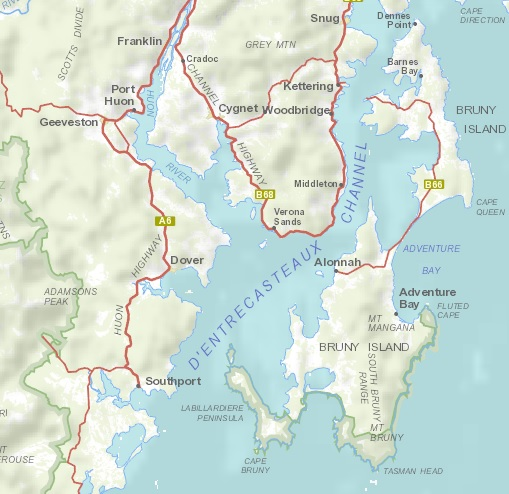
\includegraphics[width=0.7\linewidth]{images/bruny-basic}
	\caption{Bruny Island, in southern Tasmania, Australia. TODO: make a map that has expanded views to show the location on world map. QGIS, perhaps.}
	\label{fig:bruny-basic}
\end{figure}


\section{Data analysis}
In section \ref{pattens-profiles} the general properties of load profiles and how they are influenced by exogenous factors was discussed. Now, these general properties will be investigated in depth for the particular feeder in the case study.
\par
let's begin by having a simple look at the load profile over a randomly selected week.
Figure \ref{fig:simpleweek} shows a single week of apparent power draw on Bruny Island.
This was randomly selected, but is representative of a typical summer week.
Some observations are immediately obvious
\begin{itemize}
	\item The midday load is only marginally larger higher than the overnight load.
	\item Morning peaks are larger than afternoon peaks
	\item Thursday midday is much larger than any other day, in this particular week.
	\item There is some missing data on Tuesday just as the morning peak subsides.
\end{itemize}

\begin{figure}
	\centering
	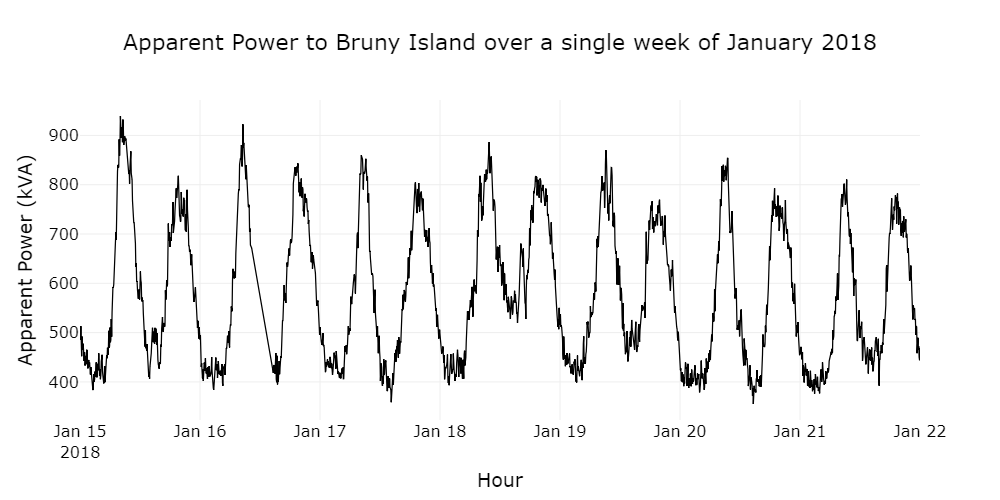
\includegraphics[width=0.7\linewidth]{images/simple-week}
	\caption{Apparent power delivered to Bruny Island over the week beginning Monday January 15, 2018}
	\label{fig:simpleweek}
\end{figure}
